\newcommand{\colorhref}[2]{\href{#1}{\color{blue}{#2}}}

In vitro, depolarization block has been shown to limit the maximum firing rate of dopaminergic (DA) neurons \cite{Richards1997}, and is caused by a sustained, large amplitude membrane current \cite{Bianchi2012}. Normally, DA neurons located in the midbrain fire in two different regimes: single spikes and bursts of action potentials. Previous studies have suggested that an imbalance between these two regimes may play a critical role in the physiopathology of schizophrenia \cite{Benamer2018}. Antipsychotic drugs used to manage schizophrenia exert their therapeutic action via depolarization-induced inactivation of midbrain dopamine cell activity \cite{Grace1997}. Therefore, understanding the way that these neurons enter into depolarization block may potentially lead to improved therapeutics \cite{Qian2014}.

Qian et al. (2014) studied depolarization block in two simplified models (3-dimensional and 2-dimensional) which are proposed reductions of a more complex 5-dimensional model. The 5D model was a single compartment model used to capture the essential features of dopaminergic entry into depolarization block. The following three currents were used: fast sodium ($I_{Na}$), delayed rectifier potassium ($I_{K}$) and leak current($I_{leak}$). The corresponding gating variables used were the activation of sodium current ($m$), the fast inactivation ($h$) and slow inactivation of sodium current ($h_s$), and the activation of potassium current ($n$). The equations governing each gating variable were comprised of voltage dependent steady-states (described by Boltzmann function) and finally, the time constants specific to the gating variables at membrane potential ($v$). The specifics of these equations can be found in Table 1 and page 2 of the original manuscript. 

Previous work had revealed that a failure to recover from sodium channel inactivation is one way to enter into depolarization block, as the availability of sodium channels limits the maximum firing rate of DA cells \cite{Qian2014, Deister2009,Kuznetsova2010}. Previous work also suggested that this unavailability of sodium channels may have been caused by a slow inactivation component of sodium channels (represented here as $h_s$) \cite{Ding2011}. Elaborating on this hypothesis, Qian et al. (2014) developed a simplified modelling framework based on a previous model. These new models, the 3D and 2D model, either included or excluded a slow inactivation term ($h_s$) respectively, to analyze the role of the slow inactivating component.

To generate the 3D and 2D models, the authors’ performed a model reduction by separation of timescales method. The activation of sodium current was very fast compared to the time course of the other state variables and so it was set to steady-state value. Next, the time constants for the activation of potassium current ($n$) and the fast inactivation of sodium current ($h$) had similar time scales, hence $n$ was set as a function of $h$ ($f(h)$). The details of this equation will be discussed in the Discussion section. As a result, the 3D model contained 3 state variables ($v$, $h$, and $h_s$), while the 2D model contained 2 state variables ($v$ and $h$) with $h_s$ set to 1 to eliminate slow inactivation. 

The authors found that while their new models matched \emph{in vitro} measurements of DA neurons; adding a slow component of sodium inactivation qualitatively changed how the model entered depolarization block. Specifically, the slow time course of inactivation allows multiple spikes prior to entry into depolarization block, and that the block (cessation in firing) occurs near or below spike threshold (-45 to -30 mV \emph{in vitro}). Interestingly, they also attempted to clarify the controversy regarding the role of NMDA and AMPA receptors, where they show that depending on the relative contributions to depolarization, these receptors can affect bursting and depolarization block in different ways. 

We aim to replicate Figures 1--4 and 6 of the original manuscript \cite{Qian2014}, (we omit their Figure 5 as it consists of experimental data). As such, our Figures 1--4 correspond to the authors' Figures 1--4, however, our Figure 5 corresponds to their Figure 6. It is important to note that we could not fully replicate all of their figures, we've discussed this with the original authors and they provided us with what code they had available. Unfortunately the code was incomplete (only contained the model definition for the 2D and 3D models), and we could not be sure if it was the final version. We compared what we had with the available code and noted that there were no significant differences other than a few differences in some of the coefficients in the equation used to reduce the 5D model. These differences are elaborated on in the Discussion section.



\section{Methods}

This replication uses the model described by Qian et al. (2014), and personal communication with the authors. While the original study computed all simulations, bifurcation diagrams, and nullclines using XPPAUT, our replication uses Python3.6 (for full package specifications including version numbers, please see the included \colorhref{https://github.com/mupsh/ReScience\_Qian\_2014/blob/master/requirements.txt}{requirements file} in the code repository). We solve the ODEs with the scipy \emph{odeint} function which is a stiffness-switching adaptive solver. $1.5\times 10^{-8}$ was used for the relative and absolute tolerance (except Figure 1C which uses $1\times 10^{-3}$ due to stiffness issues). Solutions are saved with a resolution of 0.1 ms. Additionally we used pyDSTool \cite{pydstool} for computing bifurcation diagrams, which provides a python interface to the AUTO bifurcation environment. For plots with a periodic solution, we typically discard the first 1000 ms of the solution to eliminate the transient, and in Figure 1C we discard the first half of the solution. 

Our code consists of two packages (generators and ode\_functions) used to compute the solutions. The ode\_functions package provides common tools for solving the ODE problems in the original works. The \emph{current} module contains a collection of functions for computing different types of current for each model, such as membrane current, individual ionic current, and AMPA/NMDA current. The \emph{gating} module defines all gating functions for ODEs. This includes all the gating equations that were provided in the original works. Next, \emph{diff\_eq} is a monolithic module for solving all ODE problems. It provides functionality to create 2D, 3D, and 5D ODE systems, as well as managing initial conditions. As previously noted, this module uses scipy to solve the ODEs. The \emph{experiment} module contains helpers for performing experimental manipulations including clamping, and sequences of discrete pulses. Lastly, the \emph{nullclines} module contains a collection of functions for computing nullclines and generating traces with them.

The generators package provides a module for creating each figure 1-4, and 6 from the original works. Additionally, we have a \emph{plotting}, and \emph{units} modules for generating figures, handling units. The entire implementation is run with the \emph{run} script which takes arguments as seen in the README. 

The model description is directly from page 1 and 2 of the original paper. Additionally, the model gating variables are from Table 1, and definitions for the reduced models are taken from page 3. It should also be noted that in order to get qualitatively similar results to those shown in Figure 1D2 we change the time constant equation (Table 1 of the original manuscript) for the activation of potassium current ($\tau_n$) for all simulations as follows:

\begin{center}
	$$\tau_{n^{original}} = 1 + 19 e^{- \left(\frac{\ln\left(1 + 0.05 (V+40)\right)}{0.05}\right)^{2}/300}$$
	$$\tau_{n^{modified}} = 1 + 19 e^{- \left(\frac{\ln\left(1 + 0.05 (V+60)\right)}{0.05}\right)^{2}/300}$$
\end{center}

In the equation above, the membrane potential is represented by $V$. Using the original time constant equation we found significantly different results (see \colorhref{https://github.com/mupsh/ReScience\_Qian\_2014/blob/master/figures/figure\_supp\_1D1.pdf}{Supplemental 1D1}). We noticed that the original $\tau_n$ definition contained a term $\ln\left(1 + 0.05 (v+40)\right)$ i.e. for any $V\leq-60$ this function would be undefined. Examining the original figures we can see $V$ extends past that point, we therefore (somewhat arbitrarily) set the offset to 60 giving a minimum function range of $-80$mV. While this was a guess, it yielded a model which looked qualitatively similar. 
For a summary of all replication changes, see Table \ref{tab:changes_summary}. 

\begin{table}[ht]
		\centering 
		\begin{tabular}{|l|c|c|c|}
		\hline
		& Original & Replication & Location of Change\\
		\hline
		$\tau_n$ & $1 + 19 e^{- \left(\frac{\ln\left(1 + 0.05 (V+40)\right)}{0.05}\right)^{2}/300}$ & $ 1 + 19 e^{- \left(\frac{\ln\left(1 + 0.05 (V+60)\right)}{0.05}\right)^{2}/300}$ & Everywhere\\
		\hline 
		$g_{Na}$ & 5.92nS/cm\textsuperscript{2} & 3.05mS/cm\textsuperscript{2} & Figure 1A\\
		\hline
		$g_{Na}$ & 9.12nS/cm\textsuperscript{2} & 5.92mS/cm\textsuperscript{2} & Figure 1B\\
		\hline
		Pulse Width & 3ms & 5 ms & Figure 1B\\
		\hline 
		$E_{AMPA}$ & Not specified & 0mV & Figure 5\\
		\hline
		$E_{MNDA}$ & Not specified & 0mV & Figure 5\\
		\hline
		$g_{NMDA}$ & 60nS/cm\textsuperscript{2} &  2.2$\mu$S/cm\textsuperscript{2} & Figure 5\\
		\hline
		$g_{AMPA}$ & 2.3nS/cm\textsuperscript{2} &  2.3$\mu$S/cm\textsuperscript{2} & Figure 5A\\
		\hline
		$g_{AMPA}$ &  7nS/cm\textsuperscript{2} &  7$\mu$S/cm\textsuperscript{2} & Figure 5B\\
		\hline
		\end{tabular}
		\caption{Summary of Changes}
		\label{tab:changes_summary}
	\end{table}

\section{Results}

We attempt to replicate all original figures, with the exception of Figure 5 (experimental data). Figures 1, 2 and 6 had some minor and major discrepancies, which will be addressed accordingly.

\subsection{Figure 1}
In Figure 1, the authors demonstrated the validity of their reduced 2D and 3D models. In Figure 1A they plotted the peak currents of the models with and without $h_s$ (slow sodium gating) against experimental data from \cite{Seutin2010}. This successfully showed that they had not compromised the fit of the original sodium current description to previously published data, as both models overlay the experimental data at the same points. The experiment involved repeatedly clamping $V$ to -120mV then clamping it to a new voltage for each plotted potential. For each sequential clamp the peak sodium current was measured.

For this simulation the authors specified $g_{Na}=5.92$nS/cm\textsuperscript{2} (in this work typical conductances are on the order of mS/cm\textsuperscript{2}). Using this number we create nearly 0 current (see \colorhref{https://github.com/mupsh/ReScience\_Qian\_2014/blob/master/figures/figure\_supp\_1A\_v1.pdf}{Supplemental 1A(v1)}). If we assume this was a typo and the authors meant $g_{Na}=5.92$ mS/cm\textsuperscript{2} we produce a current approximately 2 times larger than it should be (see \colorhref{https://github.com/mupsh/ReScience\_Qian\_2014/blob/master/figures/figure\_supp\_1A_v2.pdf}{Supplemental 1A(v2)}). By scaling $g_{Na}$ based taking the ratio of the peak amplitudes between the authors plot and supplemental 1A(v2), which is 0.514: we achieve Figure 1A which shows both nearly identical results for the models with and without $h_s$, and strong similarity to the original manuscript. We conclude this based on the plateau at the beginning maintaining position at 0 pA until -40 mV is reached and the downward slope toward a trough just before 0 mV is reached, followed by the upward slope toward 0 pA again. 

Next, their Figure 1B displayed the effect of slow inactivation of sodium current when a 3 ms depolarizing clamp to 0 mV was repeatedly applied to the model at 100 ms intervals from a holding potential of $-70$ mV. Again, we assume that sodium conductance should have been given in mS/cm\textsuperscript{2} and the authors specified a magnitude of $9.12$ with a depolarizing pulse width of 3 ms. Their base numbers cause a figure which does not match. Through experimentation with different amplitudes and pulse widths we settled on $g_{Na}=5.92$ and a 5 ms pulse width (for other combinations see supplemental figures \colorhref{https://github.com/mupsh/ReScience\_Qian\_2014/blob/master/figures/figure\_supp\_1B_v1.pdf}{1B(v1)}, \colorhref{https://github.com/mupsh/ReScience\_Qian\_2014/blob/master/figures/figure\_supp\_1B\_v2.pdf}{1B(v2)}, and \colorhref{https://github.com/mupsh/ReScience\_Qian\_2014/blob/master/figures/figure\_supp\_1B\_v3.pdf}{1B(v3)}). With our corrected implementation (Figure 1B), we see an initial pulse at 0 ms to -250 pA, followed by 4 pulses spaced 100 ms apart, gradually ascending to approximately -200 pA, similar to the original implementation. There are slight differences in amplitude and we assume this is due to a slightly different $g_{Na}$.

In reducing the 5D model, Qian et al. (2014) modified the potassium current activation ($n$) to a be a function of fast inactivation of sodium current ($h$) as they share similar gating kinetics. As such, $n$ was approximated by a function of $h$ i.e. ($f(h)$) where $0\leq f(h)\leq 1$. $f$ was defined as a cubic function, with coefficients for the polynomial using a least-squares fit. This was shown in their Figure 1C where $f(h)$ was compared to the limit cycle projected onto the $n, h$ phase space. In our replication (Figure 1C) does not match the authors', which is not surprising considering that we're using a modified $\tau_n$ as explained above. However, importantly, the voltage waveforms (Figures 1D1 and 1D2) are nearly identical to the authors', implying that the ultimate dynamics are comparable. 

Figures 1D1 and 1D2 compared the 5D model to the 3D model respectively. This is well replicated with our implementation (Figures 1D1 and 1D2). The peaks all occur at approximately 10 mV and troughs occur at approximately -70 mV, as well as the same timescale of pacemaking events. It is important to note that Figure 1D1 (5D model) used the modified time constant equation for the activation of sodium current. Supplemental Figure 1D1 shows the pacemaking activity with the original time constant equation, where the troughs are rounded and look considerably different from the original works (see \colorhref{https://github.com/mupsh/ReScience\_Qian\_2014/blob/master/figures/figure\_supp\_1D1.pdf}{Supplemental 1D1}).

\begin{figure}
	\centering
	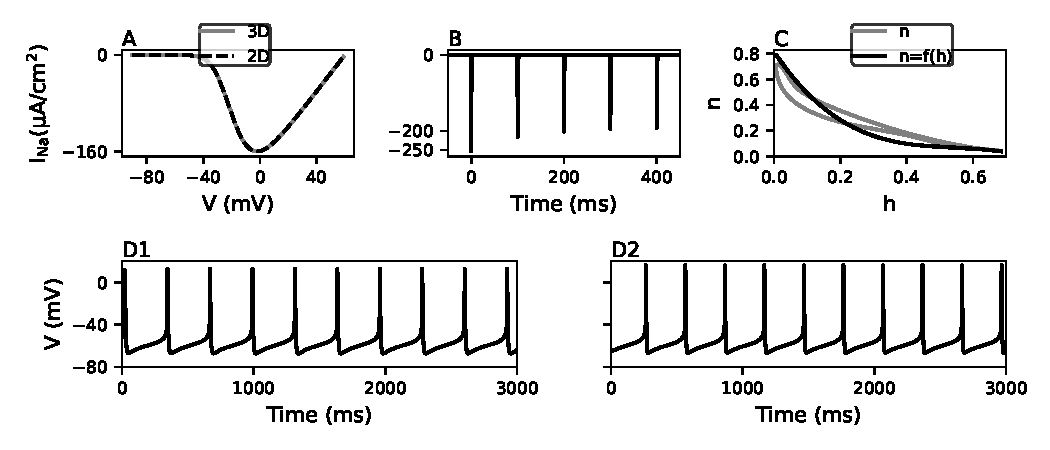
\includegraphics[scale=0.7]{../figures/figure_1.pdf}
	\caption{Replication of model development and reduction. A: Peak sodium voltage-clamp currents with and without $h_s$ are identical. B: Slow inactivation of the sodium current with repeated 5-ms depolarizing pulses to 0 mV applied at 100-ms intervals from a holding potential of -70 mV. C: The activation of potassium current ($n$) and the modified potassium current ($f(h)$) plotted against the fast inactivation of sodium current ($h$). D1: The 5D model. D2: The reduced 3D model, of note is the similarity to D1.}
	\label{fig:1}
\end{figure}

\subsection{Figure 2}

Figure 2 of the original implementation analyzed a depolarization event using the 2D model (without $h_s$). Their Figure 2A demonstrated that applying a current step caused a ``ringing'' (increase in frequency and decrease in amplitude) just before entry into depolarization block (stabilized at -19 mV), with their voltage scale ranging from -50 mV to 20 mV. We observe this same ``ringing'' in our replication (Figure 2A), however it is significantly shorter in terms of event length. Additionally, our voltage scale ranges from -70 mV to 40 mV. Without access to their original code, it is hard to conclude why we see this discrepancy especially since part A and B of this figure reuse the same code for the model implementation, and part B looks correct. However, we show the same qualitative results - i.e. ringing prior to entry into depolarization block.

The authors' Figures 2B1 and 2B2 were a nullcline analysis of $h$ with an applied current of 0 $\mu$A/cm\textsuperscript{2} and 3.5 $\mu$A/cm\textsuperscript{2} respectively. Our replications of both show identical results, demonstrated in our Figures 2B1 and B2. In Figure 2B1 we see the same shape of the V-nullcline maximum where the unstable fixed point is located at the same point of intersection, and the slope of the h-nullcline is the same. In Figure 2B2, again we see the same shape of the V-nullcline with the stable fixed point located at the same point of intersection, and the slope of the h-nullcline is the same.

\begin{figure}
	\centering
	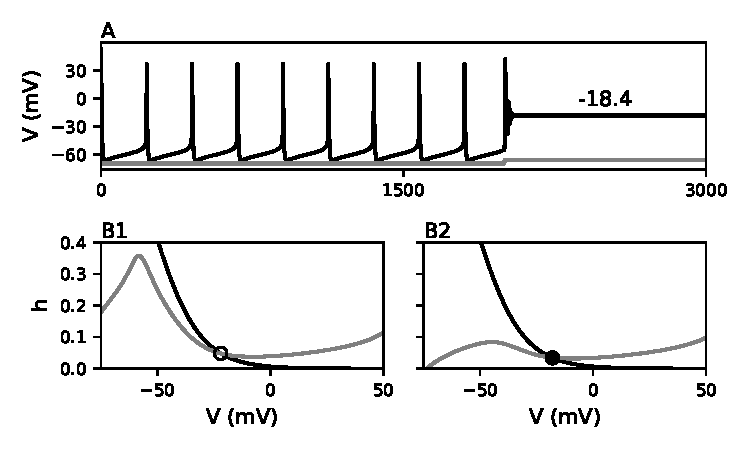
\includegraphics[scale=0.7]{../figures/figure_2.pdf}
	\caption{Entry into depolarization block using the 2D model. A: A 3.5 $\mu$A/cm\textsuperscript{2} current step (grey line) applied from 0 $\mu$A/cm\textsuperscript{2} causing entry into depolarization block (close-up shown in the upper right corner). B1: The V-nullcline (grey line) and the h-nullcline (black line) intercept at an unstable fixed point (open circle) when the applied current is 0 $\mu$A/cm\textsuperscript{2}. B2: The V-nullcline and the h-nullcline intersect at a stable fixed point (closed circle) with an applied current of 3.5 $\mu$A/cm\textsuperscript{2}.}
	\label{fig:2}
\end{figure}

\subsection{Figure 3}
Qian et al. (2014) then analyzed the entry into depolarization block with the 3D model. Their Figure 3A1 plotted membrane current of the 3D model followed by an applied current causing depolarization block. They demonstrated that slow inactivation of sodium current provided a mechanism for spike frequency adaptation as opposed to the ``ringing'' seen with the 2D model. Our implementation, shown in Figure 3A1, replicates this well. We see the same increase in oscillation frequency post-stimulus, as well as the same instantaneous frequencies for each interspike interval leading up to depolarization block (overlaid with right axis). In Figure 3A2 the authors investigated the contribution of $h_s$ to $h_{total}$ (defined as $h_{total}= h_{s}\cdot h$) with the same applied current seen in Figure 3A1. This is also well replicated in our Figure 3A2, which demonstrates large oscillations in $h_s$ and $h_{total}$ at the beginning of the time course, which then decrease in amplitude and frequency post-stimulus, followed by a cessation in firing at the end of the time course.

\begin{figure}
	\centering
	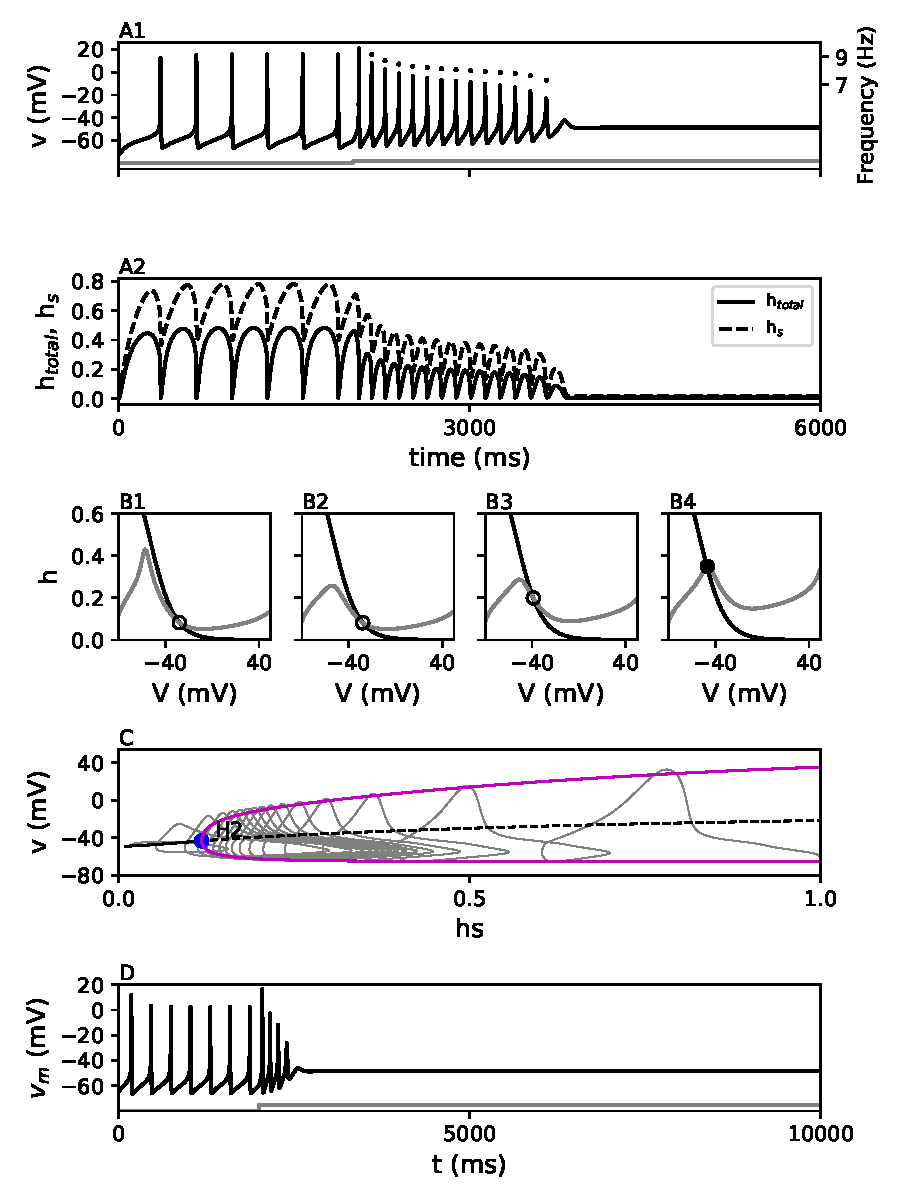
\includegraphics[scale=0.7]{../figures/figure_3.pdf}
	\caption{Entry into depolarization block using the 3-D model. A1: Membrane current with an applied current of 0.16 $\mu$A/cm\textsuperscript{2} from 0 $\mu$A/cm\textsuperscript{2} causing entry into depolarization block. The filled circles show the instantaneous frequency for each interspike interval before entering depolarization block. A2: Contribution of $h_s$ (dashed line) to $h_{total}$ (solid line; $h_{total}= h_{s} \times h$) with an applied current of 0.16 $\mu$A/cm\textsuperscript{2} from 0 $\mu$A/cm\textsuperscript{2} causing entry into depolarization block. B1--B4: V-nullcline (grey line) and the h-nullcline (black line) intersect at different unstable (open circle) and stable (closed circle) fixed points in response to different applied currents and $h_s$ constants. B1: Applied current of 0 $\mu$A/cm\textsuperscript{2} and $h_s$ set to 0.6. B2: Applied current of 0.16 $\mu$A/cm\textsuperscript{2} and $h_s$ set to 0.6. B3: Applied current of 0.16 $\mu$A/cm\textsuperscript{2} and $h_s$ set to 0.2. Applied current of 0.16 $\mu$A/cm\textsuperscript{2} and $h_s$ set to 0.05. C: Bifurcation analysis with $h_s$ as the bifurcation parameter. From left to right: stable fixed point (black line), trajectory (light grey line), Hopf (blue circle, H2), oscillatory extrema (pink line), and the unstable fixed point (dashed line). D: Same as A1 but with slow inactivation sped up by a factor of 2 ($dh_s/dt \rightarrow 2dh_s/dt$).}
	\label{fig:3}
\end{figure}

In Figures 3B1--B4 the authors also performed a nullcline analysis and outlined the effects of varying the current stimulus and $h_s$. The $h_s$, and bias current parameters were taken from characteristic regimes in Figure 3A2 (pre-stimulus, amplitude decay, amplitude plateau, and cessation). Our results, shown in Figures 3B1--B4, replicate their results well. In each nullcline analysis we see the same position and shapes of the maxima of the V-nullcline and the same consistent slope of the h-nullcline. The points of intersection with the three unstable points and one stable point corresponding to B1--B3 and B4 respectively, are all located at the same location as the original works. 

Similarly, Figures 3C and 3D are well replicated. 3C was a bifurcation analysis with $h_s$ as the bifurcation parameter overlaid with the trajectory. Here we see the same location of the supercritical Hopf bifurcation, the same slight slope of the stable fixed point, as well as the same unique trajectory shape throughout. 3D shows the results of speeding up slow inactivation of sodium current by a factor of 2, where we have a faster convergence toward the fixed point and fewer spikes, as seen in the original implementation.



\subsection{Figure 4}
Next, the authors used Figure 4 to compare the differences between the 2D and the 3D model, thereby analyzing the significance of the slow inactivation of sodium current. Figure 4A1 and 4B2 show the effect of moving the V-nullcline in the 2D and 3D models respectively (summarizing the analysis performed in Figure 2B and 3B1--B4). Our results (Figure 4A) have the same shapes and slopes of the nullclines as well as the location of the stable and unstable fixed points when compared to the original implementation. To follow that, Qian et al. (2014) then compared the bifurcation analysis of the 2D model and 3D model in Figures 4B1 and 4B2. Our replication (Figure 4B) replicates the stable oscillation, unstable oscillation, unstable fixed points, and fixed points. We also have the same key features noted by the authors, being the three branches of fixed points to the left of the pacemaking region in Figure 4B1, and the single branch of fixed points in Figure 4B2. Of note is a difference in naming conventions: the authors' use SNP (saddle node of periodic), our implementation uses LPC (limit point of cycles).

Lastly, the original works produced current-voltage (I-V) curves as they are more familiar to electrophysiologists. Their Figure 4C1 was the nonmonotonic IV curve (2D model) which is required for a saddle node bifurcation to initiate spiking \cite{Qian2014}, and their Figure 4C2 was the monotonic IV curve (3D model) which the authors’ had noted was often associated with a Hopf bifurcation for spike initiation. They used these figures to show that monotonic curves should be produced with voltage clamp steps on the order of seconds or with very slow ramp current, and conversely, nonmonotonic curves should be produced with fast ramps that do not allow sufficient slow inactivation of the sodium channel current. We replicate these in our Figures 4C1 and 4C2 by clamping the voltage and computing the membrane current across voltage steps. There are slight differences in the zero-crossing point, and scale of the I-V curves between our implementation and the authors. This could arise from the authors using a slightly non-standard definition of I-V curve, or slightly different parameters. 

\begin{figure}
	\centering
	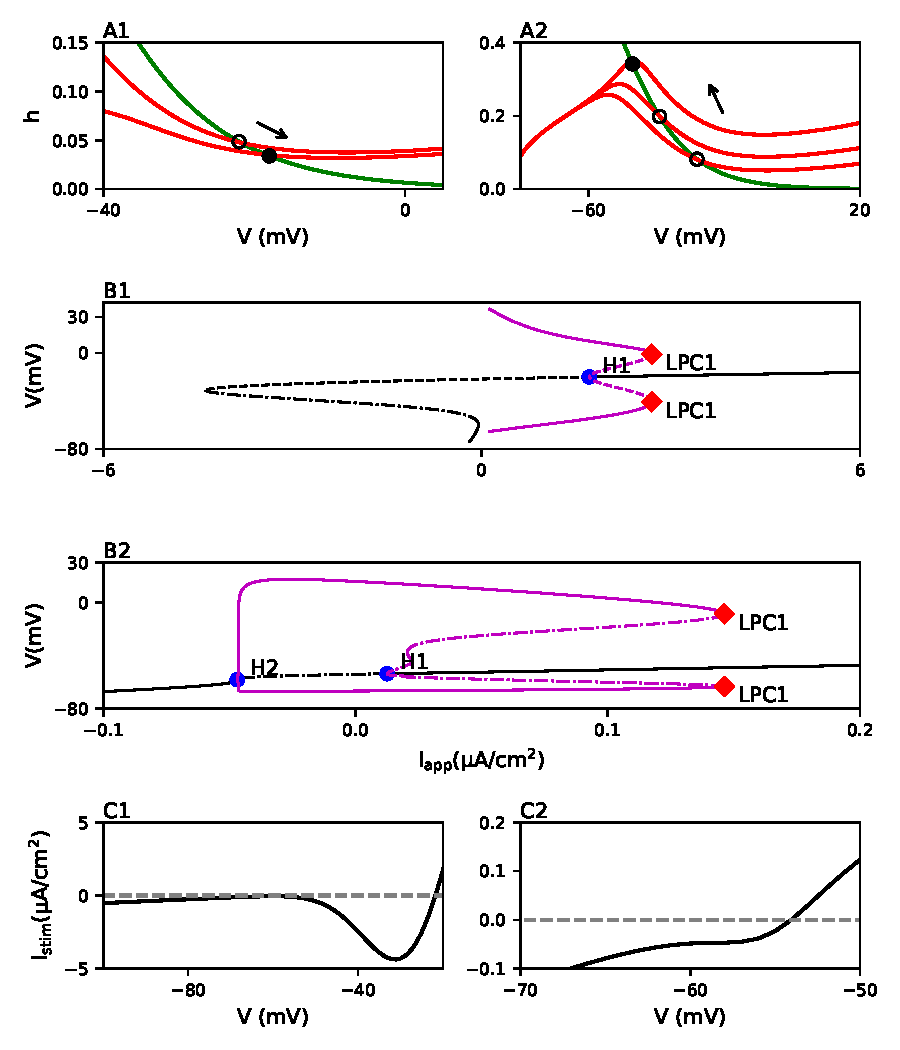
\includegraphics[scale=0.7]{../figures/figure_4.pdf}
	\caption{A1: The V-nullcline (red) and the h-nullcline (green) for the 2D model as the applied current is increased from 0 to 3.5 $\mu$A/cm\textsuperscript{2} from left to right as denoted by the arrow. The unstable points and stable fixed points are denoted using the open circles and closed circles respectively. A2: The voltage nullcline (red) and the $h$ nullcline (green) for the 3-D model as $h_s$ is decreased from 0.6 to 0.2 to 0.05 from right to left as denoted by the arrow. B1: Bifurcation diagram for the 2D model showing 3 branches of fixed points to the left of the pacemaking region. C1: nonmonotonic I-V curve for the 2D model. C2: monotonic I-V curve for the 3D model. \textbf{Legend for bifurcation}. H1, H2 indicates the Hopf, LPC1 indicate the limit points. Pink lines are limit cycles, and black lines are nodes with dashed, and solid lines representing unstable and stable regimes respectively.}
	\label{fig:4}
\end{figure}


\subsection{Figure 5}
Finally, the authors studied the effects of NMDA and AMPA currents on the entry into depolarization block. As we did not duplicate Figure 5 (experimental data), their Figure 6 corresponds to our Figure 5. Their Figure 6 demonstrated that the activation of NMDA receptors can delay entry into depolarization block, but activation of AMPA receptors cannot. They used these receptors as a more physiologically relevant method of depolarization of dopamine neurons. The authors’ mentioned that in previous literature there had been some controversy as to the role of these receptors in depolarization block, and so they examined how the activation of these receptors interacted with the slow inactivation of the sodium channel in their model. In the original works, their Figures 6A1, A2, and A3 displayed the results for the minimal NMDA current, AMPA current, or injected current required to induce depolarization block in the 3D model. Unfortunately they did not specify the reversal potentials for $E_{AMPA}$, or $E_{NMDA}$ so we assume they were set to 0 mV - as is common \cite{neuroscience_2001}. We replicate the current pulse portion of this figure using the 3D model (shown in our Figure 5A1--A3), where we see the same style of frequency increase until depolarization block occurs around -48 mV (Figure 5A3). However, we used different parameters for the channel conductance since the parameters specified by the authors (on the order of nS/cm\textsuperscript{2}) were insufficient to introduce depolarization block. We started with their given parameters (2.3, and 60) assuming the correct unit was mS/cm\textsuperscript{2} and then sequentially scaled the constant until we achieved results which were similar in appearance. As a result the conductance value of $g_{AMPA}$ was modified from 2.3 nS/cm\textsuperscript{2} to 2.3 $\mu$S/cm\textsuperscript{2}. Similarly the NMDA conductance value was changed from 60 nS/cm\textsuperscript{2} to 2.22 $\mu$S/cm\textsuperscript{2}. Although the replication is not perfect, we still see most of the same key features with a longer delay of entry into depolarization block post-stimulus. However, depolarization block occurs at a higher value of -50 mV rather than their result of -43 mV in the case of NMDA

Next, the author’s compared the same three manipulations at a constant final level of depolarization in order to focus on the effect of linearity versus nonlinearity of the activated conductance. With their results, they concluded that NMDA receptors delayed entry into depolarization block due to the nonlinearity of the NMDA conductance which allows it to compensate for the slow inactivation of sodium current. Conversely, they concluded that AMPA receptors have linear conductance which favours depolarization block.  Our replication (Figure 5B1-3) originally had the same issues as seen in Figure 5A. However, when we applied the same scale factor to the AMPA and NMDA conductance values as we had applied in 5A, we obtained similar results. Figure 5B1 is the same as Figure 5A1, and therefore the NMDA conductance value as well as the results and their inconsistencies are the same. Our AMPA conductance value (again converting the 7 nS/cm\textsuperscript{2} to 7 $\mu$S/cm\textsuperscript{2}) produces very similar results to the authors' original, with the same increase in spike frequency and relatively fast entry to depolarization block. Differently however, depolarization block itself occurs around -44 mV rather than their result of -43 mV (Figure 5B2). Lastly, Figure 6B3 is well replicated in our Figure 5B3, where entry into depolarization block happens relatively quickly.

\begin{figure}
	\centering
	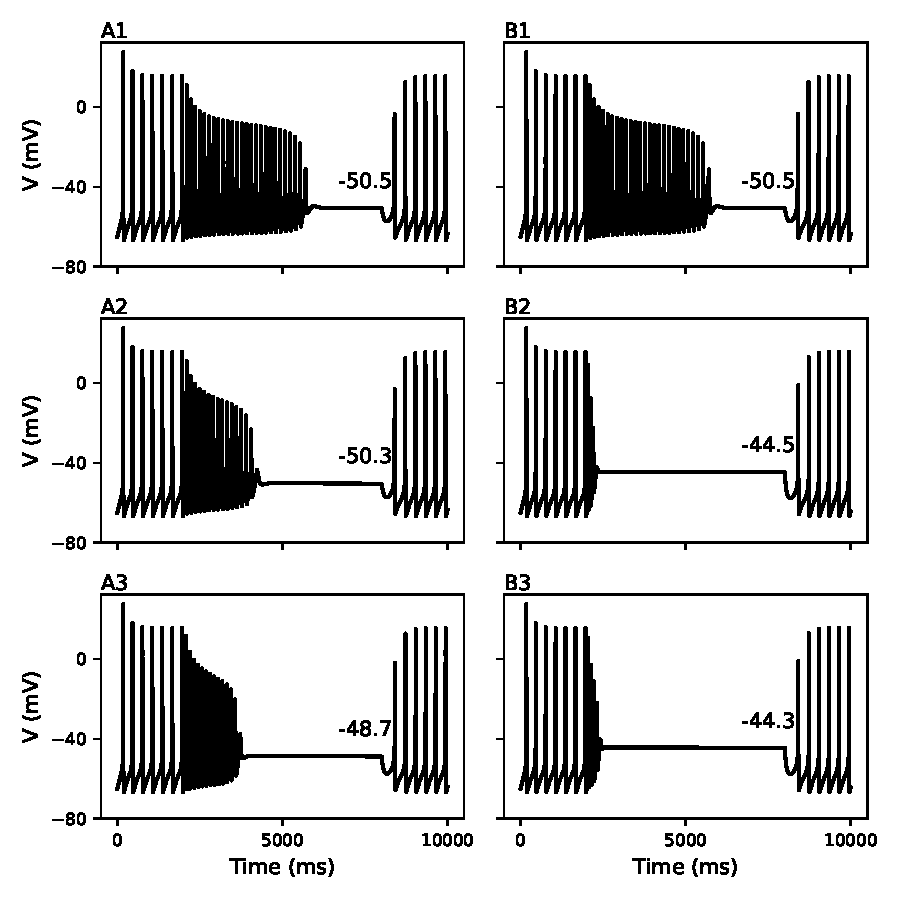
\includegraphics[scale=0.7]{../figures/figure_6.pdf}
	\caption{A1-A3: Square pulses of conductance or current applied to the 3-D model. A1: NMDA conductance pulse of 2.22 $\mu$S/cm\textsuperscript{2}. A2: AMPA conductance pulse of 2.3 $\mu$S/cm\textsuperscript{2}. A3: Applied current pulse of 0.16 $\mu$A/cm\textsuperscript{2}. B1-B3: Comparison of square pulses that were supposed to induce the same level of depolarization as seen in Figure 6 A1-A3 of the original works. B1: NMDA conductance pulse of 2.22 $\mu$S/cm\textsuperscript{2}. B2: AMPA conductance pulse of 7 $\mu$S/cm\textsuperscript{2}. B3: Applied current pulse of 0.32 $\mu$A/cm\textsuperscript{2}. }
	\label{fig:6}
\end{figure}


\section{Discussion}

Overall, this implementation replicates the original paper. There are some inconsistencies with the 5D model (Figure 1), the 2D model (Figure 2) and with the analysis using NMDA receptors (Figure 6 of the original works). Upon speaking with the authors, they kindly provided us with one of their XPP files for the 3D model but unfortunately did not have the 5D model or the AMPA model. As previously mentioned, we found some discrepancies when replicating Figure 1C which we were able to partially restore by modifying $\tau_n$ (see Methods). The polynomial, $f(h)$ = $a_0 + a_1 + a_2 + a_3$ was used in the reduction of the model as described in the Methods section.  The original constants for $f(h)$ were $a_0 =0.8158$, $a_1= −3.8768$ $a_2 = 6.8838$, and $a_3 = −4.2079$. The constants provided by the ODE file were $a_0 = 0.8437$, $a_1 = -4.1480$, $a_2 = 7.5234$, and $a_3 = -4.6486$. While the authors’ ODE file contained a different set of constants for $f(h)$, when we ran the model with the new constants, we found negligible qualitative and quantitative differences. Thus, the modified equation seems to be the best way to restore the proper model fit given in the original paper. Additionally, the AMPA model was absent from the provided XPP file, therefore we could not cross-reference with their published model or verify the differences we found using our implementation. Although we could not be sure that our model was quantitatively implemented correctly, it was the closest solution to restoring the qualitative features of their AMPA model. Lastly, we were unable to ascertain the reversal potential of either AMPA and NMDA in their XPP file or the manuscript, therefore we assume them both to be 0 mV \cite{neuroscience_2001}. Next, our Figure 2A has a shorter and less prominent ``ringing'' period when entering depolarization block and there is a discrepancy with the voltage scale. Our scale ranges from -70 mV to 40 mV and their scale ranged from -50 mV to 20 mV.  Despite this, the cessation in firing still occurs around -19mV as demonstrated in the original implementation and has identical spike shapes prior to depolarization block. Lastly, our findings when originally replicating Figure 6 were dramatically different from that of the initial implementation. With the provided ODE file, it was unclear which conductances were used in the model. Seeing as the bifurcation analysis replicated in our Figures 3 and 4 were nearly identical to theirs (strongly implying very similar if not identical dynamics), we do not believe the issue was in the model specification. Given their description we were unable to replicate Figure 6, the reason being that we believe that the authors provided incorrect parameters. Taking this into consideration, we manipulated the NMDA and AMPA conductances. Using this technique, we were able to achieve quantitatively similar depolarization block for AMPA, but only qualitative behaviour in the NMDA model

Despite the discrepancies, our implementation by far demonstrates that all the major qualitative, and scientific results using the 2D and 3D models were implemented correctly in the original works, if only slightly mis-represented in the parameters used of the original manuscript.
